%\documentclass[handout]{ximera}
\documentclass[nooutcomes]{ximera}

\usepackage{gensymb}
\usepackage{tabularx}
\usepackage{mdframed}
\usepackage{pdfpages}
%\usepackage{chngcntr}

\let\problem\relax
\let\endproblem\relax

\newcommand{\property}[2]{#1#2}




\newtheoremstyle{SlantTheorem}{\topsep}{\fill}%%% space between body and thm
 {\slshape}                      %%% Thm body font
 {}                              %%% Indent amount (empty = no indent)
 {\bfseries\sffamily}            %%% Thm head font
 {}                              %%% Punctuation after thm head
 {3ex}                           %%% Space after thm head
 {\thmname{#1}\thmnumber{ #2}\thmnote{ \bfseries(#3)}} %%% Thm head spec
\theoremstyle{SlantTheorem}
\newtheorem{problem}{Problem}[]

%\counterwithin*{problem}{section}



%%%%%%%%%%%%%%%%%%%%%%%%%%%%Jenny's code%%%%%%%%%%%%%%%%%%%%

%%% Solution environment
%\newenvironment{solution}{
%\ifhandout\setbox0\vbox\bgroup\else
%\begin{trivlist}\item[\hskip \labelsep\small\itshape\bfseries Solution\hspace{2ex}]
%\par\noindent\upshape\small
%\fi}
%{\ifhandout\egroup\else
%\end{trivlist}
%\fi}
%
%
%%% instructorIntro environment
%\ifhandout
%\newenvironment{instructorIntro}[1][false]%
%{%
%\def\givenatend{\boolean{#1}}\ifthenelse{\boolean{#1}}{\begin{trivlist}\item}{\setbox0\vbox\bgroup}{}
%}
%{%
%\ifthenelse{\givenatend}{\end{trivlist}}{\egroup}{}
%}
%\else
%\newenvironment{instructorIntro}[1][false]%
%{%
%  \ifthenelse{\boolean{#1}}{\begin{trivlist}\item[\hskip \labelsep\bfseries Instructor Notes:\hspace{2ex}]}
%{\begin{trivlist}\item[\hskip \labelsep\bfseries Instructor Notes:\hspace{2ex}]}
%{}
%}
%% %% line at the bottom} 
%{\end{trivlist}\par\addvspace{.5ex}\nobreak\noindent\hung} 
%\fi
%
%


\let\instructorNotes\relax
\let\endinstructorNotes\relax
%%% instructorNotes environment
\ifhandout
\newenvironment{instructorNotes}[1][false]%
{%
\def\givenatend{\boolean{#1}}\ifthenelse{\boolean{#1}}{\begin{trivlist}\item}{\setbox0\vbox\bgroup}{}
}
{%
\ifthenelse{\givenatend}{\end{trivlist}}{\egroup}{}
}
\else
\newenvironment{instructorNotes}[1][false]%
{%
  \ifthenelse{\boolean{#1}}{\begin{trivlist}\item[\hskip \labelsep\bfseries {\Large Instructor Notes: \\} \hspace{\textwidth} ]}
{\begin{trivlist}\item[\hskip \labelsep\bfseries {\Large Instructor Notes: \\} \hspace{\textwidth} ]}
{}
}
{\end{trivlist}}
\fi


%% Suggested Timing
\newcommand{\timing}[1]{{\bf Suggested Timing: \hspace{2ex}} #1}




\hypersetup{
    colorlinks=true,       % false: boxed links; true: colored links
    linkcolor=blue,          % color of internal links (change box color with linkbordercolor)
    citecolor=green,        % color of links to bibliography
    filecolor=magenta,      % color of file links
    urlcolor=cyan           % color of external links
}

\title{Circular Trigonometry}
\author{Bart Snapp and Brad Findell}

\outcome{Learning outcome goes here.}

\begin{document}
\begin{abstract}
We investigate how trigonometric functions relate to circles.
\end{abstract}
\maketitle

\begin{teachingnote}
Need Trigonometry Checkup as preactivity, perhaps with a special office hour.  

Remind students of sine, cosine, and tangent in terms of $x$, $y$, and $r$ in the first quadrant.  

Given an angle, the approach is to pick an $x$ and $y$ that work and to see that the trig ratios should be independent of the choice.  

A key point here is ``extending the domain of an idea.''  Some things no longer work the same way.
\end{teachingnote}

As we have seen, right triangle trigonometry is restricted to acute angles.  But angles are often obtuse, so it is quite useful to extend trigonometry to angles greater than $90^\circ$.  Here is one approach:  Place the angle with the vertex at the origin in the coordinate plane and with one side of the angle (the initial side) along the positive $x$-axis.  
Measure to the other side of the angle (the terminal side) as a counter-clockwise rotation about the origin.   

\begin{image}
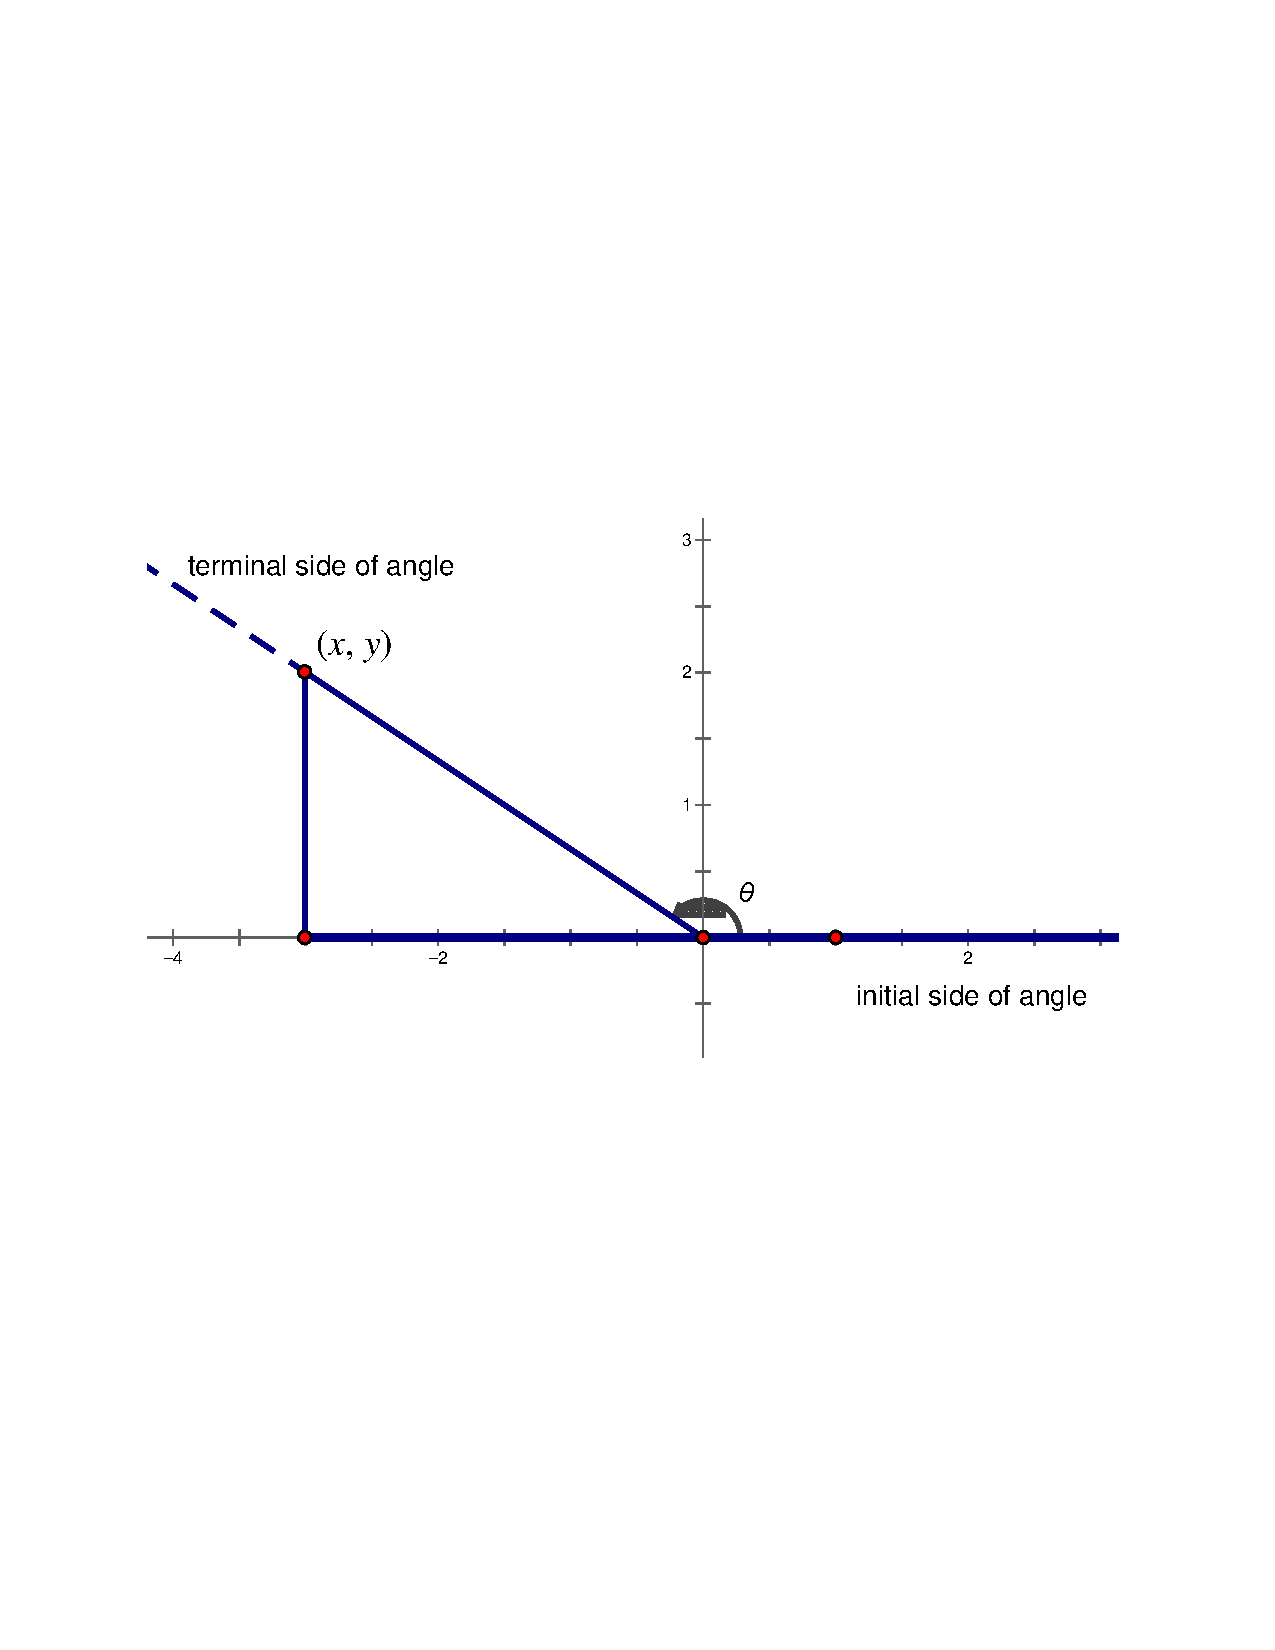
\includegraphics[scale=0.6]{referenceTriangle}
\end{image}

If we choose a point on the terminal side of this angle, we can draw what is called \emph{reference triangle} by dropping a perpendicular to the $x$-axis.  Then we can use the values of $x$, $y$, and $r$ from this triangle, just as before.  What is different in this picture is that $x$ is negative, as will be the case for any angle with a terminal side in the second quadrant.  


\begin{problem}
Draw a picture and use it to find the following values: 
\begin{enumerate}
\item $\sin 135^\circ = $
\item $\cos 135^\circ =$
\item $\tan 135^\circ =$
\end{enumerate}
\vfill
\end{problem}

\newpage

\begin{problem}
Draw a picture and use it to find the following values: 
\begin{enumerate}
\item $\sin 150^\circ =$
\item $\cos 150^\circ =$
\item $\tan 150^\circ =$
\end{enumerate}
\vfill
\end{problem}

\begin{problem}
For some angles, the reference triangle is not actually a `triangle,' but that's okay.  Draw pictures to demonstrate the following: 
\begin{enumerate}
\item $\sin 90^\circ =$
\item $\cos 90^\circ =$
\item $\tan 90^\circ =$
\item $\sin 180^\circ =$
\item $\cos 180^\circ =$
\item $\tan 180^\circ =$
\end{enumerate}
\vfill
\end{problem}

%\begin{problem}
%Now we can find the area of a triangle given two sides and an angle.\standardhs{G-SRT.9}  
%\end{problem}
%% Laws of Sines and Cosines \standardhs{G-SRT.10}, \standardhs{G-SRT.11}

Because angles are often about rotation, angles greater than $180^\circ$ can make sense, too.  And negative angles can describe rotation in the opposite direction.  If we consider the angle to change continuously, then rotation about the origin creates a situation that repeats every $360^\circ$.  This repetition provides the foundation for modeling lots of repetitive (periodic) contexts in the real world.  For this modeling, we need \emph{circular trigonometry}, which turns out to be much cleaner if (1) angles are measured not in degrees but in a more ``natural'' unit, called radians; and (2) we use \emph{the unit circle}, which is a circle of radius 1 centered at the origin.   

\newpage

\begin{problem}
Below is the unit circle with special angles labeled in degrees, radians, and with 
coordinates.\margincomment{CCSS F-TF.2. Explain how the unit circle in the coordinate plane enables the
  extension of trigonometric functions to all real numbers,
  interpreted as radian measures of angles traversed counterclockwise
  around the unit circle.}
\begin{image}
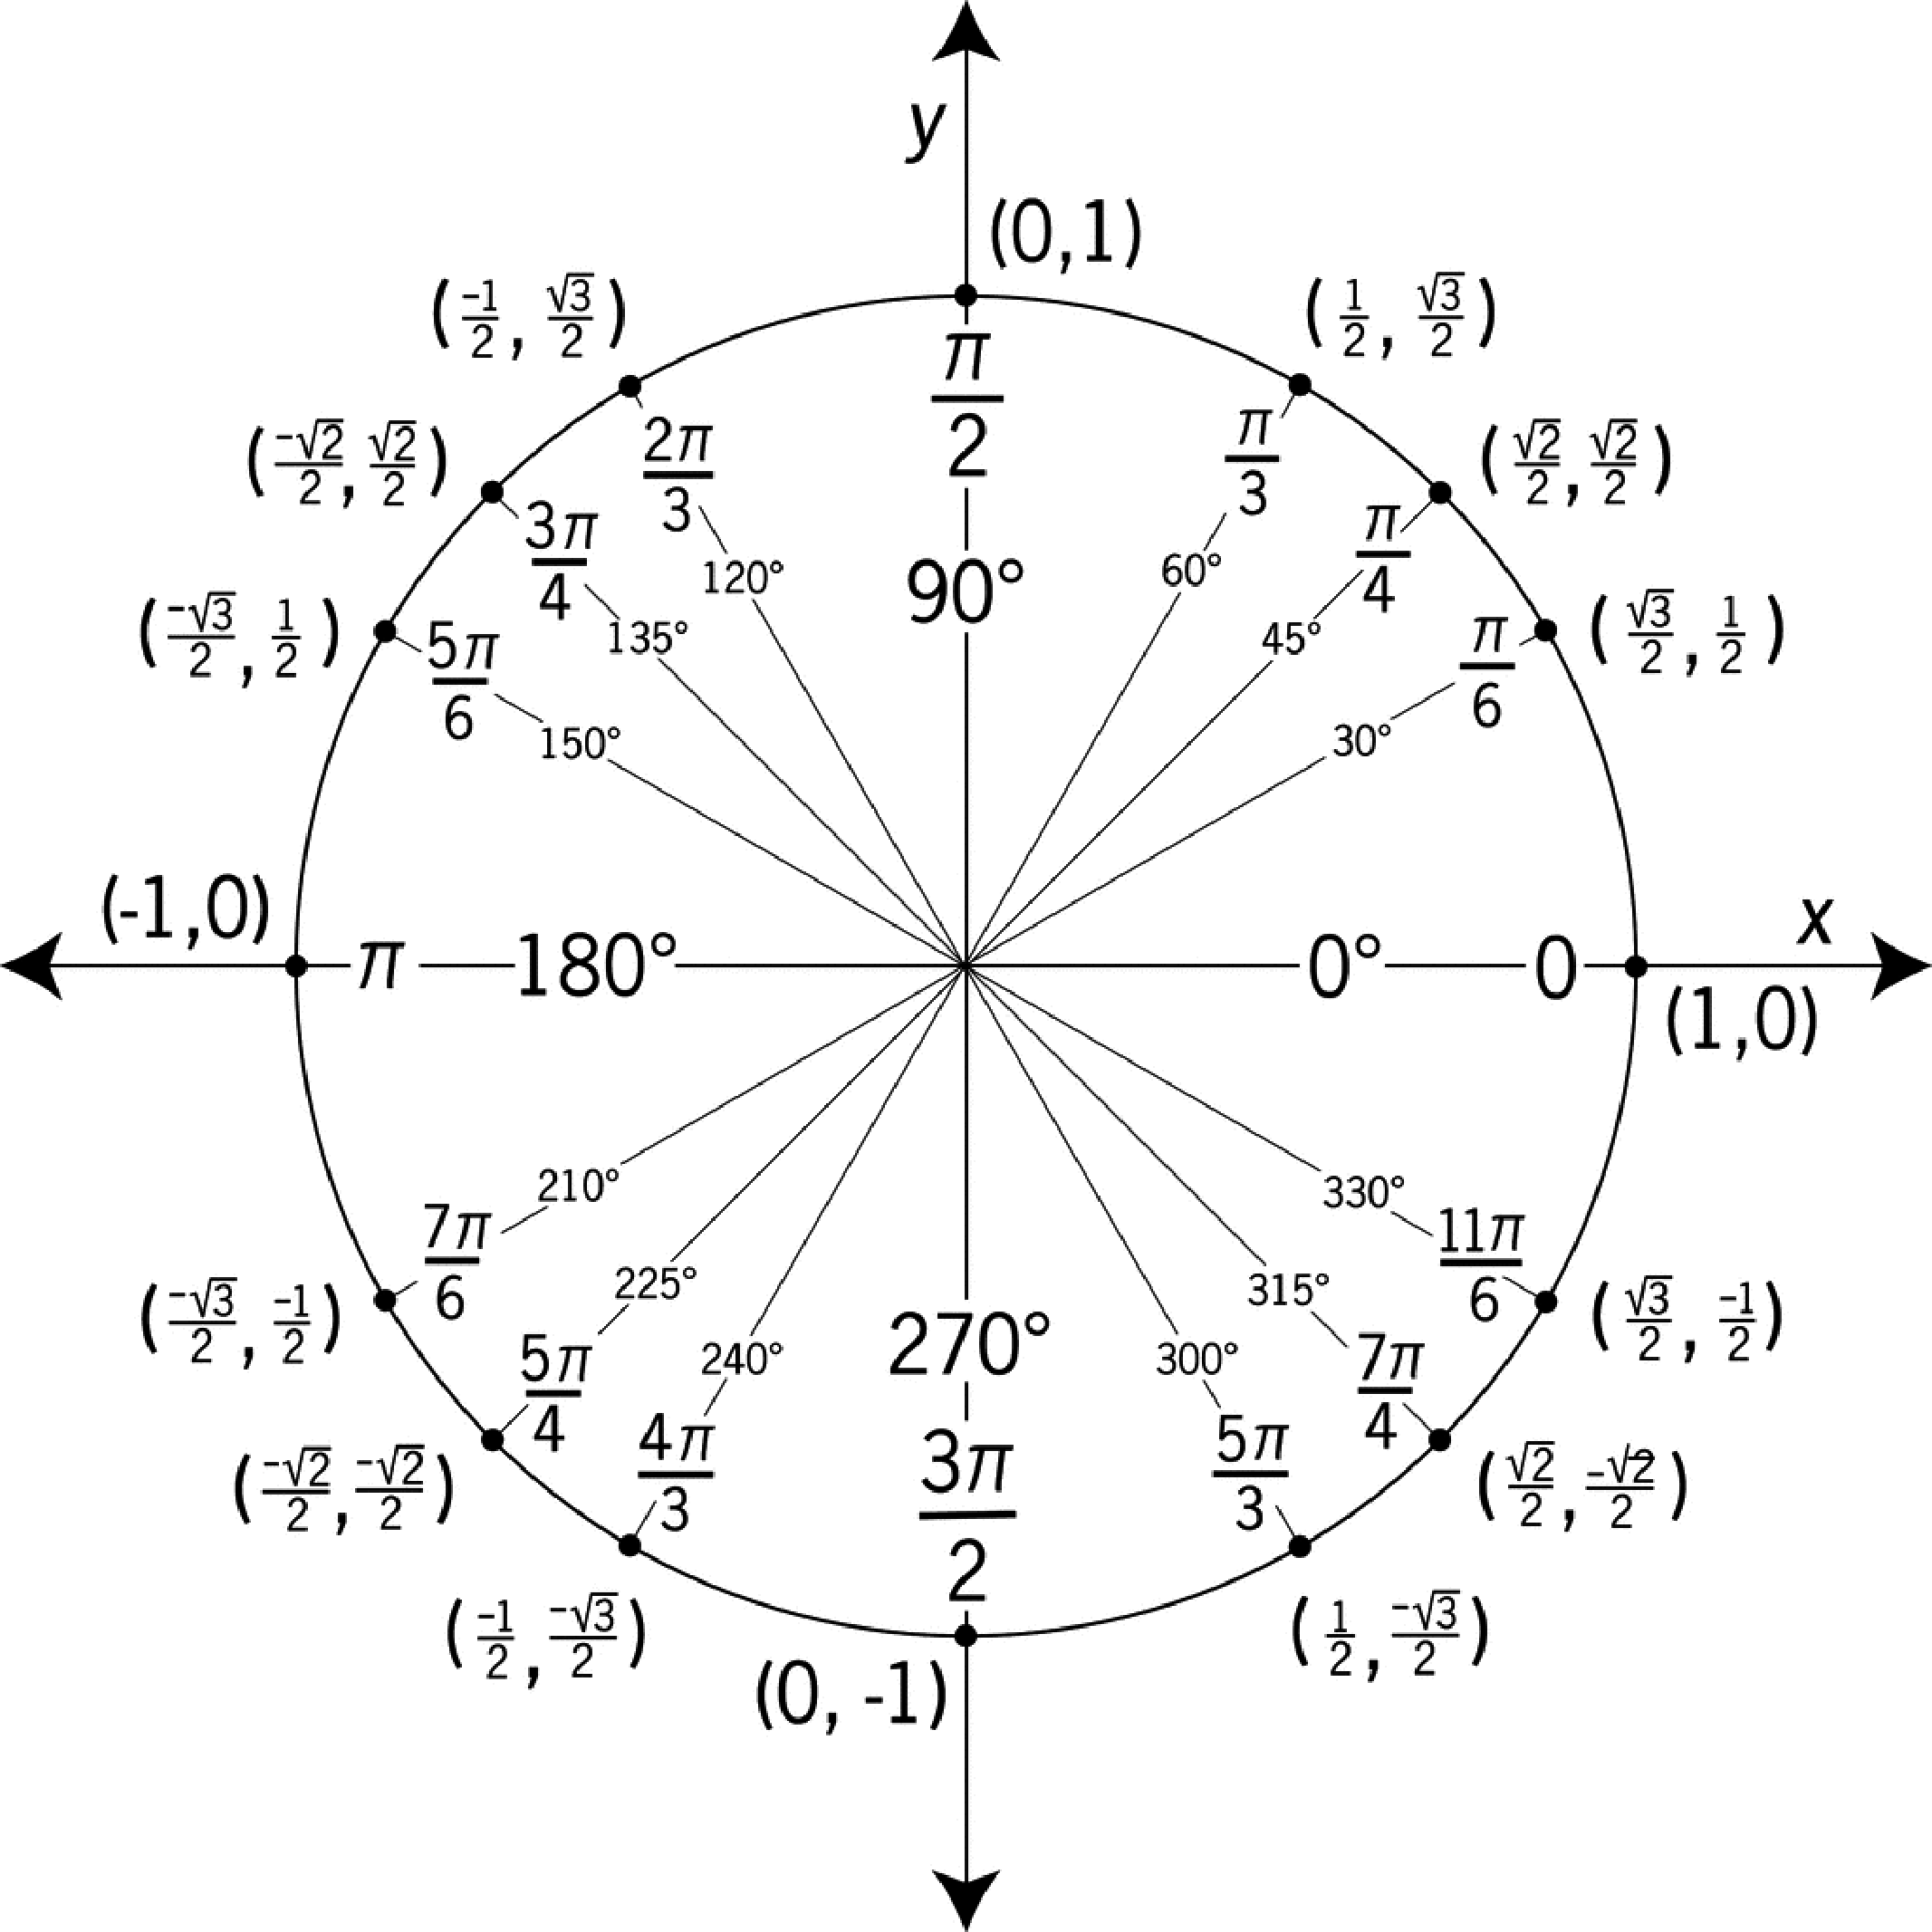
\includegraphics[scale=0.25]{unitCircle.pdf}
\end{image}
\begin{enumerate}
\item Explain what the various numbers mean in this unit circle.  
\item Use the unit circle to make a table showing (1) angle in degrees, (2) angle in radians, (3) sine of the angle, and (4) cosine of the angle.  
\item Use your table to draw a graph of $\sin\theta$ versus $\theta$.
\item Use your table to draw a graph of $\cos\theta$ versus $\theta$.
\item Explain why it makes sense to connect the dots. 
\item Extend your graphs to angles greater than $360^\circ$, and use the unit circle to explain why your extension makes sense. 
\item Extend your graphs to angles less than $0^\circ$, and use the unit circle to explain why your extension makes sense.
\end{enumerate}
\vfill
\end{problem}

\begin{teachingnote}
Now is a good time to explore modeling with trig functions and to develop radian measure.  
\end{teachingnote}

%\begin{enumerate}
%\item Understanding radian measure.\standardhs{G-C.5}, \standardhs{F-TF.1}
%
%\item Using the unit circle to extend trigonometry to angles of any measure.\standardhs{F-TF.2}
%
%\item Choosing and using trig functions to model periodic phenomena.\standardhs{F-TF.5}
%\item Fluency finding trig functions of special angles in radian measure.\standardhs{F-TF.3}
%
%\end{enumerate}

\end{document}
